\chapter{SoPC}
------------------------


\section{Avalon Memory Mapped Interface}
The Avalon Memory Mapped (Avalon MM) interface is used throughout the project to interconnect
blocks with memory elements and the SoPC interconnect. An example Avalon MM waveform
is shown in Figure \ref{figure:avalonmm}.
\begin{figure}[h!]
\begin{center}
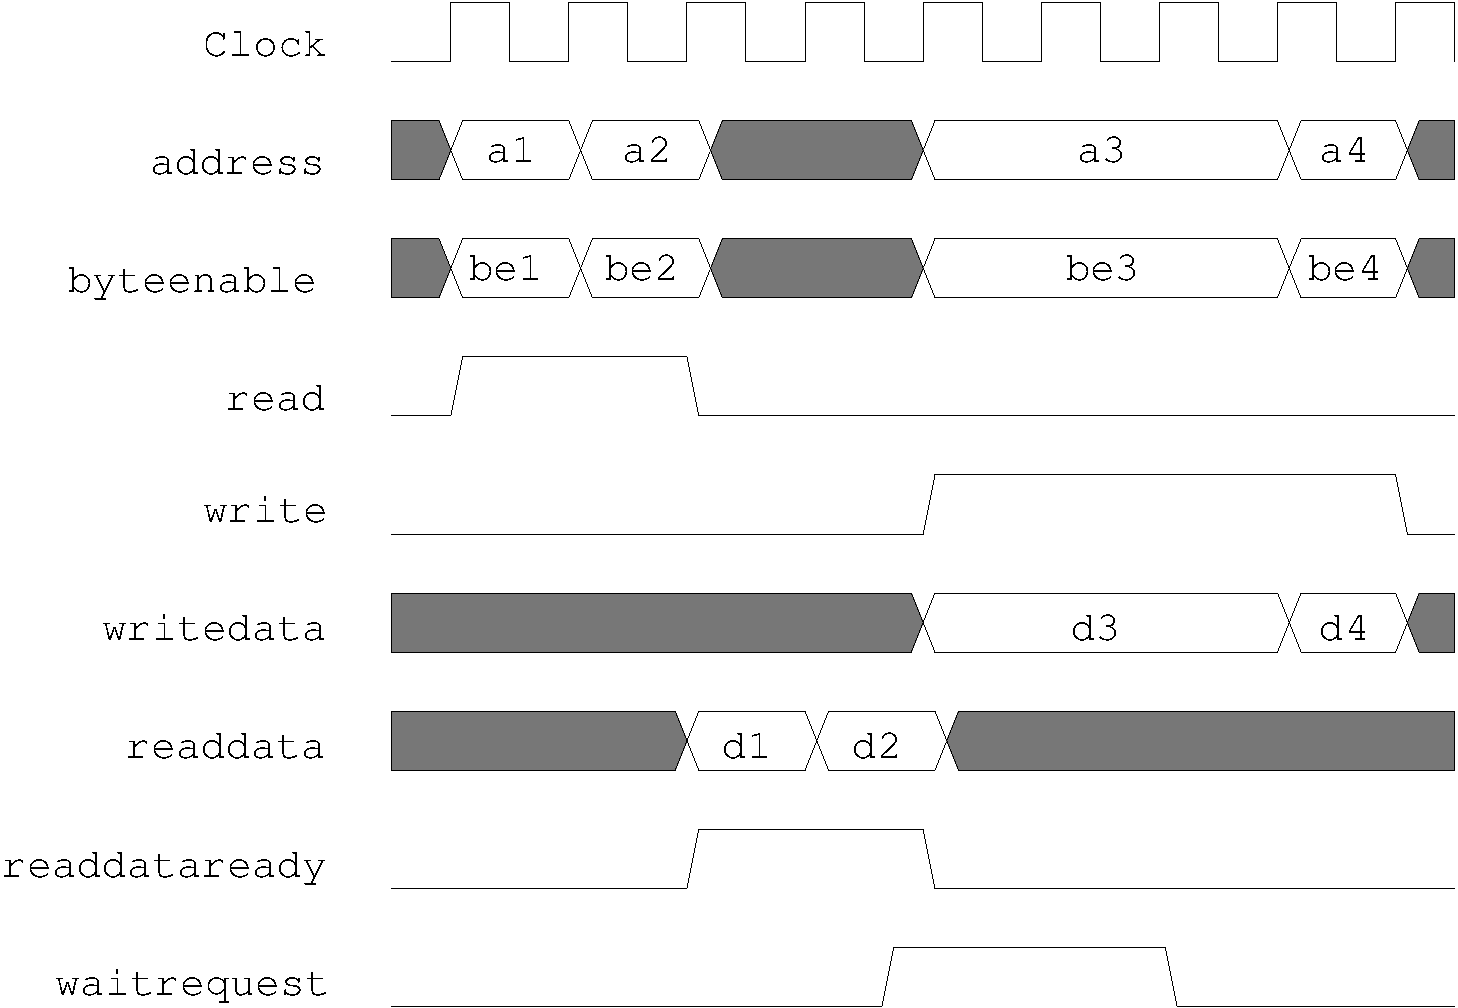
\includegraphics[width=0.95\textwidth]{avalonmm}
\caption{Example waveforms of an Avalon MM bus}
\label{figure:avalonmm}
\end{center}
\end{figure}


The master can issue both reads and writes, which a slave then replies to. A read
is initiated by setting the desired address and byte enables and asserting the \texttt{read}
signal. The master can continue issuing reads to different addresses as long as the \texttt{waitrequest}
signal stays low. If the Avalon MM slave asserts the \texttt{waitrequest} signal, the master needs
to hold the current signals for as long as the \texttt{waitrequest} signal is asserted.
The Avalon MM slave will reply to the read by asserting the \texttt{readdataready} signal
and providing the requested read data on the \texttt{readdata} bus.

Similarly writes are initiated by the Avalon MM master by setting the desired address, byte enables,
data to write and asserting the \texttt{write} signal. The master can assume that the write completed
without waiting any further unless the \texttt{waitrequest} signal is asserted, in which case,
similarly to the reads, the master needs to hold the signals steady until \texttt{waitrequest} is deasserted.

% XXX: some simulation waveforms?


\newpage
\section{Overview}
A decision was made to use a hybrid software and hardware approach to tackle the problem
so as to simplify the required hardware. To achieve this, a system on programmable chip
(SoPC) generated by the Altera QSys software was used.

Figure \ref{figure:sopc_overview} shows an overview of the SoPC module. The system consists of a Nios II/f core
and a number of peripherals interconnected via the QSys (Merlin) Network-on-Chip
interconnect.

\begin{figure}[h!]
\begin{center}
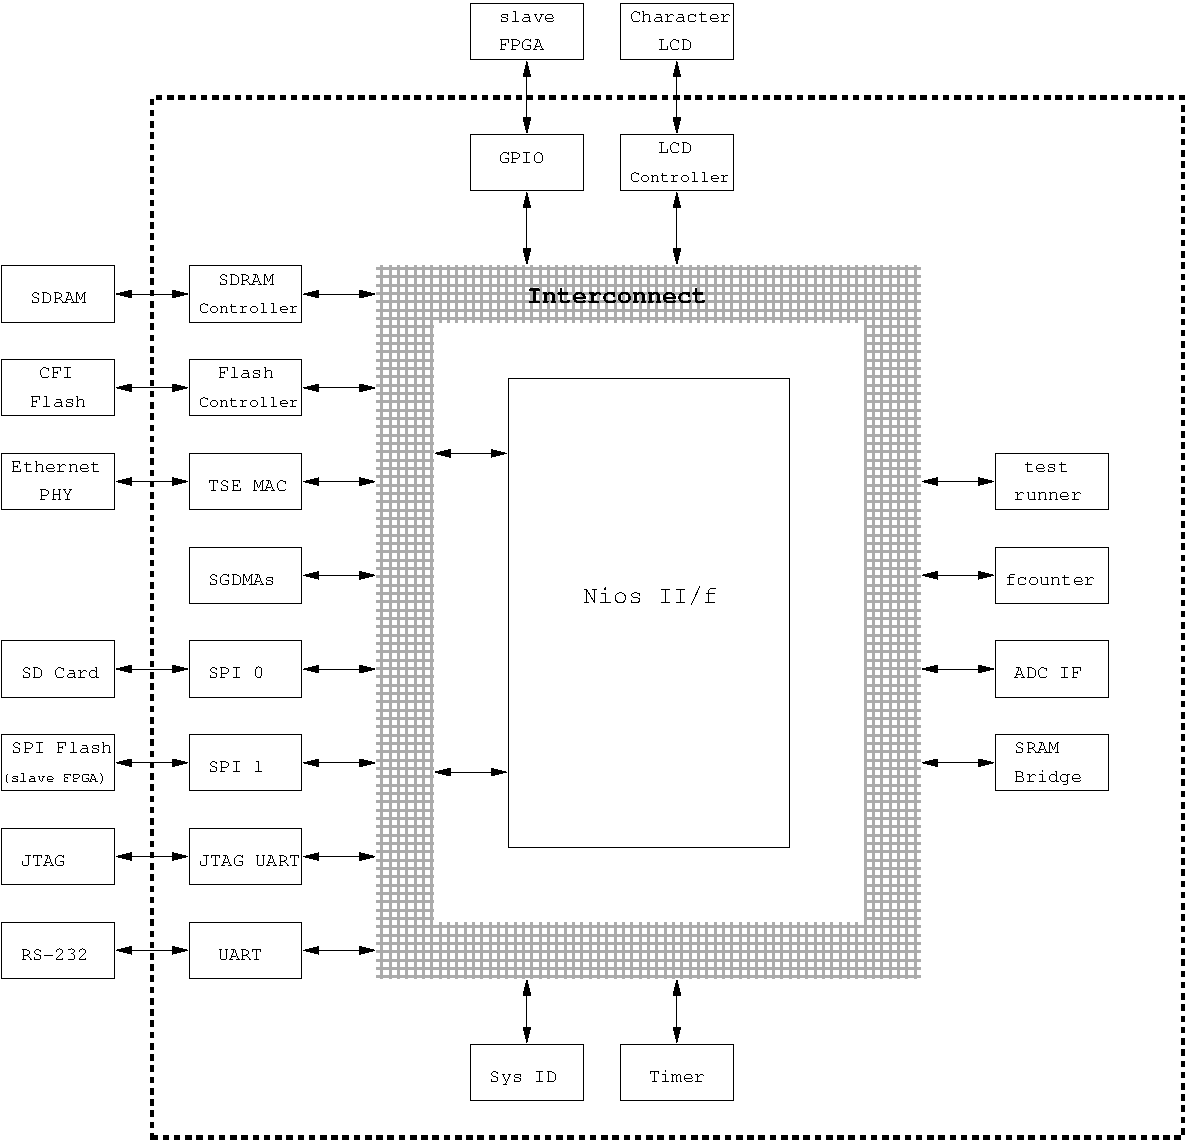
\includegraphics[width=\textwidth]{sys}
\caption{Overview of the SoPC}
\label{figure:sopc_overview}
\end{center}
\end{figure}

The system is clocked by a 100 MHz clock generated by a PLL. Additionally a 10 MHz clock
is also generated, which is used to clock the GPIO controller and the LCD controller. The
system consists of both third-party and own IP cores.

The GPIO controller provides a General Purpose I/O interface to the operating system. It
is connected to the configuration-related pins of the slave FPGA - \texttt{nCE, nSTATUS,
CONF\_DONE, nCONFIG}.

Two SPI interfaces master controllers are also included in the system. Both run the SPI
interface at a safe 10 MHz clock frequency. SPI0 is connected to the SD Card, while SPI1
connects to the SPI Flash on the slave FPGA board.

Serial connectivity is provided by the JTAG UART and UART modules. The JTAG UART
provides a serial UART interface over the USB JTAG for use with the custom Nios II software
tools on a host PC. The UART module provides a regular serial interface to the on-board
RS-232 connector. The controller implements the RX and TX signals as well as transmission control
signals CTS and RTS.

The two main memory interfaces are an SDRAM controller interfacing to the on-board 128 MB
SDRAM, and a flash controller interfacing to the on-board 8 MB CFI Flash.

An ethernet interface is provided via the Altera Triple-Speed Ethernet (TSE) MAC module. The
CPU interfaces to the TSE MAC via two Scatter-Gather DMA controller to maximize throughput. The
MAC uses an RGMII interface to connect to the on-board Ethernet PHY. The RX clock to the MAC
initially used a 0 degree phase shift. This resulted in a large number of dropped packages and
hence TCP rentransmissions. Increasing the phase shift to 90 degrees significantly improved
the receive performance. Another large improvement in transmit and receive reliability and
throughput was achieved by disabling the statistics counters in the MAC.

The system also includes a timer module for use with the operating system, and a sysid module
which provides a programmable ID and the synthesis date of the system to the operating system.

A custom module (SRAM Bridge) is used to interconnect the CPU with the internal SRAM synchronizing
arbiter (\texttt{sram\_arb\_sync}). It is only a bridge exposing a memory range as an external
Avalon MM master interface.

Further custom modules interface with other on-chip peripherals. The Test Runner module
interfaces the tester and test controller with the system. The ADC interface provides a control
interface for the on-chip ADC controller.

A custom frequency counter module takes an external signal bus, and is able to measure the frequency
on any of the incoming signals.

Table \ref{table:memorymap_cpu} shows the memory map as seen from the CPU.

\begin{table}[h!]
\centering
\begin{tabular}{ | l | l | }
 \hline
   Address Range           & Peripheral\\
 \hline
   \texttt{0x00000000 - 0x07ffffff} & SDRAM \\
 \hline
   \texttt{0x08001000 - 0x08001fff} & TSE MAC SGDMA Descriptor Memory \\
 \hline
   \texttt{0x08002800 - 0x08002fff} & JTAG Controller \\
 \hline
   \texttt{0x08003000 - 0x080033ff} & Triple-Speed Ethernet MAC \\
 \hline
   \texttt{0x08003400 - 0x0800343f} & TSE MAC SGDMA (TX) \\
 \hline
   \texttt{0x08003440 - 0x0800347f} & TSE MAC SGDMA (RX) \\
 \hline
   \texttt{0x08003480 - 0x0800349f} & Timer \\
 \hline
   \texttt{0x080034a0 - 0x080034af} & PLL \\
 \hline
   \texttt{0x080034b0 - 0x080034b7} & JTAG UART \\
 \hline
   \texttt{0x0a000000 - 0x0a7fffff} & CFI Flash \\
 \hline
   \texttt{0x0b000010 - 0x0b00001f} & LCD Controller \\
 \hline
   \texttt{0x0b000200 - 0x0b00020f} & GPIO (nSTATUS) \\
 \hline
   \texttt{0x0b000210 - 0x0b00021f} & GPIO (CONF\_DONE) \\
 \hline
   \texttt{0x0b000220 - 0x0b00022f} & GPIO (nCONFIG) \\
 \hline
   \texttt{0x0b000230 - 0x0b00023f} & GPIO (nCE) \\
 \hline
   \texttt{0x0ba00000 - 0x0ba00007} & SYS ID \\
 \hline
   \texttt{0x0ba10000 - 0x0ba1001f} & SPI 0 \\
 \hline
   \texttt{0x0ba20000 - 0x0ba2001f} & SPI 0 \\
 \hline
   \texttt{0x0c000000 - 0x0c1fffff} & SRAM (SRAM Bridge) \\
 \hline
   \texttt{0x0d000000 - 0x0d0000ff} & Test Runner \\
 \hline
   \texttt{0x0d100000 - 0x0d10001f} & UART \\
 \hline
   \texttt{0x0d200000 - 0x0d2003ff} & Frequency Counter \\
 \hline
   \texttt{0x0d300000 - 0x0d3000ff} & ADC Interface \\
 \hline
\end{tabular}
\caption{Memory map of the SoPC as seen from the CPU data master}
\label{table:memorymap_cpu}
\end{table}


\newpage
\section{Nios II}
A Nios II/f is the application processor in the SoPC. The Nios II/f is a 32-bit MIPS-based
RISC processor with a branch predictor, barrel shifter, hardware multiplication and division,
instruction and data caches and an MMU.

The choice of the Nios II/f was made in particular with the MMU in mind. The lower-end Nios II/e and
Nios II/s cores do not support an MMU. By using an MMU it is possible, by using virtual memory,
to allocate for example large buffers, of which only the used pages will be backed by real memory. For example
a 1 MB buffer will not be fully allocated with backing memory immediately, but only when all its pages are
actually used. Another important advantage of an MMU is the memory protection. Faults in userland such as
segmentation faults can be caught and recovered from.

To improve the performance of the system with an MMU, a Translation Lookaside Buffer (TLB) of 128 entries was
also included.

During the initial stages of development, the CPU was used with a Level 3 debug module, which includes a number
of hardware breakpoints and watchpoints. This was later reduced to a Level 1 debug module which only includes
a small JTAG controller.

The reset vector of the CPU points to the first location of the CFI Flash, so that the CPU boots up from
the non-volatile Flash memory. The exception vectors are located in the SDRAM, where the OS will be located
as soon as the bootloader has loaded it.

Initially a small cache size of just 4kB and 8kB (with a line size of 32 bytes) was chosen for
the D and I caches respectively. Given the large amount of unused resource on the board a decision
was made to increase those sizes to 32kB and 64kB respectively. Table \ref{table:benchmark} shows some benchmark results
with both cache sizes. The improvement is fairly significant. In the case of Dhrystone, the complete
benchmark fits into the caches with the new larger cache sizes.


\begin{table}[h!]
\centering
\begin{tabular}{ | l | r | r | }
 \hline
   Benchmark           & Score (small caches) & Score (large caches)\\
 \hline
   Dhrystone & 92165.9 & 119617.2 \\
 \hline
   BYTEmark Numeric Sort & 26.574 & 33.36 \\
 \hline
   BYTEmark String Sort & 1.3667 & 1.8123 \\
 \hline
   BYTEmark Bitfield & 5.6997e+06 & 5.8613e+06 \\
 \hline
\end{tabular}
\caption{Benchmark results for small and large caches respectively}
\label{table:benchmark}
\end{table}



\newpage
\section{Test Runner}
The test runner module provides a memory-mapped interface to control the external
tester module. Figure \ref{figure:tr_blackbox} shows an overview of the signals of this core.
\begin{figure}[h!]
\begin{center}
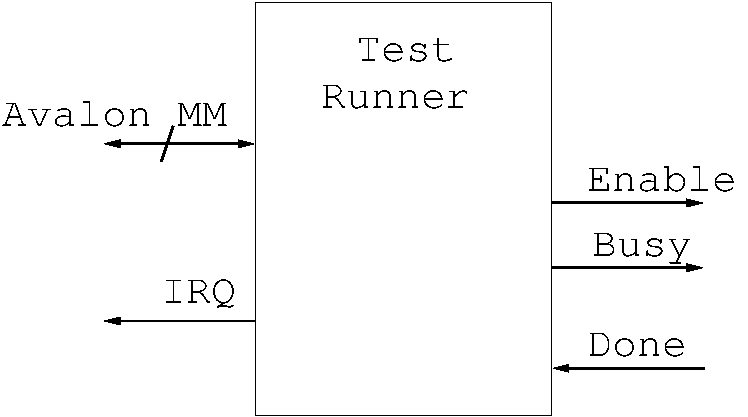
\includegraphics[width=0.4\textwidth]{tr}
\caption{Black box overview of Test Runner}
\label{figure:tr_blackbox}
\end{center}
\end{figure}


The Avalon MM Slave interface connects to the SoPC and provides a convenient
memory-mapped interface to its internal registers. The interrupt sender interface
connects directly to the interrupt controller of the CPU.

The peripheral bus consists of three signals: a \texttt{busy} signal which feeds as
one of the select signals into the SRAM Arbiter (\texttt{sram\_arb\_sync}), a \texttt{enable}
signal and a \texttt{done} signal which connect to the \texttt{tester} module.

Table \ref{table:trunner_memorymap} shows the memory map of the core. The system can read an ID from the
ID register (which always contains the hexadecimal value 0x0a) to verify that
the device is responding. A write to the enable register will assert the peripheral
\texttt{enable} line for one cycle. A read of the done register returns the value
of the \texttt{done} peripheral signal.

When a rising edge occurs on the \texttt{done} signal, the IRQ register is written
and the IRQ line to the CPU is asserted. As soon as the IRQ register is read, it is
automatically cleared and the IRQ line is deasserted.

The \texttt{busy} signal is asserted between the rising edge of the \texttt{enable} signal
and the rising edge of the \texttt{done} signal.


\begin{table}[h!]
\centering
\begin{tabular}{ | l | l | }
 \hline
   Address       & Description \\
 \hline
   \texttt{0x0a} & IRQ Register \\
 \hline
   \texttt{0x7f} & ID Register \\
 \hline
   \texttt{0x80} & Done Register \\
 \hline
   \texttt{0x81} & Enable Register \\
 \hline
\end{tabular}
\caption{Relative memory map of the test runner module}
\label{table:trunner_memorymap}
\end{table}


\newpage
\section{ADC Interface}
The ADC interface has the exact same interfaces as the Test Runner module as shown
on Figure \ref{figure:adc_if_blackbox}. The only difference is its memory map, which is slightly different
and shown in Table \ref{table:adc_memorymap}.

\begin{figure}[h!]
\begin{center}
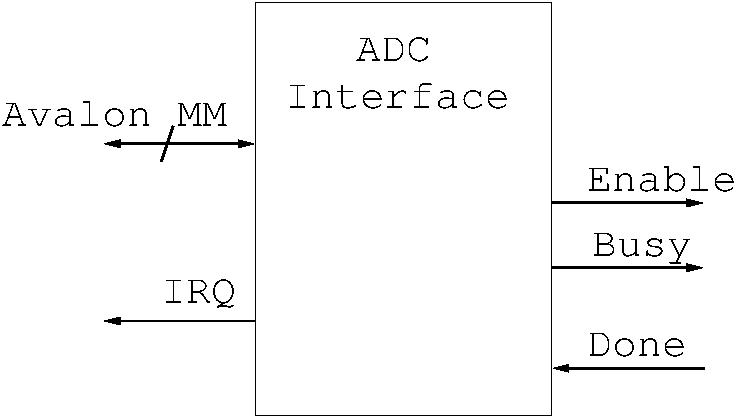
\includegraphics[width=0.4\textwidth]{adc_if}
\caption{Black box overview of Test Runner}
\label{figure:adc_if_blackbox}
\end{center}
\end{figure}

\begin{table}[h!]
\centering
\begin{tabular}{ | l | l | }
 \hline
   Address       & Description \\
 \hline
   \texttt{0x0a} & IRQ Register \\
 \hline
   \texttt{0x0f} & ID Register \\
 \hline
   \texttt{0xa0} & Done Register \\
 \hline
   \texttt{0xb0} & Enable Register \\
 \hline
\end{tabular}
\caption{Relative memory map of the adc interface module}
\label{table:adc_memorymap}
\end{table}


\newpage
\section{Frequency counter}
The frequency counter peripheral provides a simple memory-mapped interface to
measure the frequency on an input signal. Figure \ref{figure:fcounter_blackbox}
shows a black box view of the module.

\begin{figure}[h!]
\begin{center}
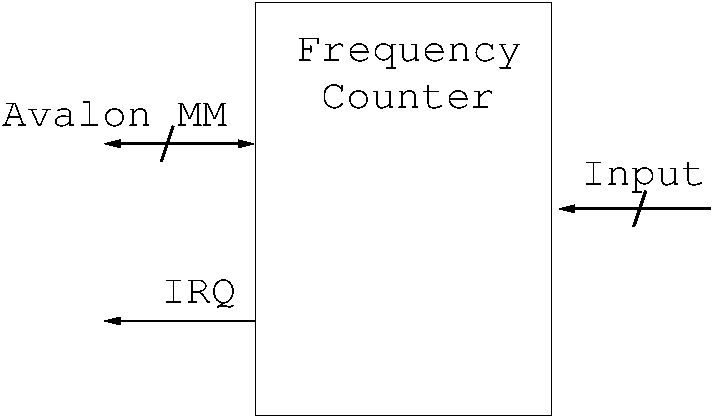
\includegraphics[width=0.4\textwidth]{fcounter_periph}
\caption{Black box overview of the frequency counter module}
\label{figure:fcounter_blackbox}
\end{center}
\end{figure}

The frequency counter consists
of three modules, a $N-to-1$ multiplexer, the measurement module and a control module.

The input bus is normally connected to the 24 outputs of the chip under test. The
multiplexer multiplexes the input bus onto a single internal signal using a select signal
which is reconfigurable via software. This allows for measurement of clock frequency
on any of the Superchip outputs without any hardware modifications.

In order to avoid metastability, since the input signal is effectively crossing a
clock domain, the design contains a synchroniser stage, to synchronise the input signal
with the FPGA clock.

During operation, the frequency counter will count the number of rising edges on the
input signal over a configurable number of cycles of the system clock.

The number of cycles over which
the edges on the input signal are measured is configurable via software to any value up
to $2^{32}$ cycles. After reset this value is $2^{23}$ cycles.

Once the module has gone through the required clock cycles, it stops counting input signal
edges and an $count\_overflow$ flag is raised which results in an interrupt being raised
from the control module.

By knowing both the number of system clock cycles over which measurement took place
and the number of edges of the input clock to be measured that occured over the same
period, it is possible to determine the ratio of the system frequency to the input
frequency. Since the system frequency is known, the input frequency can be determined.


\paragraph{Control Module}
The frequency counter control module handles the communication and the input setup
data from the processor, as well as the the output data from the measurement module.
It provides an Avalon Memory Mapped slave interface for communication with the
NIOS II processor as well as an Avalon Interrupt sender interface (\texttt{IRQ}).

Table \ref{table:fcounter_memorymap} shows the relative memory map of the frequency
counter module.


\begin{table}[h!]
\centering
\begin{tabular}{ | l | l | }
 \hline
   Address       & Description \\
 \hline
   \texttt{0x00} & Input select Register \\
 \hline
   \texttt{0x02} & Edge count Register \\
 \hline
   \texttt{0x03} & Cycle (timeout) count Register \\
 \hline
   \texttt{0x04} & IRQ Register \\
 \hline
   \texttt{0x05} & ID Register \\
 \hline
   \texttt{0x0A} & Enable Register \\
 \hline
\end{tabular}
\caption{Relative memory map of the frequency counter module}
\label{table:fcounter_memorymap}
\end{table}



The Cycle (timeout) count register determines the number of system
clock cycles over which the frequency is measured.

The ID register contains a constant used by the driver to verify the functioning
of the module.

The input select register is wired to the select input of the input multiplexer. This
register determines which input line is measured.

The edge count register is the output of the frequency counter. It contains the number
of input clock edges counted during the measurement interval. This register is valid
after an interrupt has been raised.

A write to the enable register initiates the counting operation.

The IRQ register is set to 1 when the counting operation completes. Reading from
the IRQ register will clear it. The interrupt line \texttt{IRQ} is held high
while the IRQ register is not cleared, notifying the CPU of the completed operation.


\paragraph{Resolution and Performance}
The module was designed to be able to measure frequencies according to specification
for the academic year $2011-12$ D2 Superchip' ring oscillators.
These oscillators have a basic frequency of $1MHz$ and an offset frequency of the teams' ID number
multiplied by $250kHz$ \citep{Southampton:2011:spec}. For $16$ teams, the frequency
range would be $1250kHz - 5000kHz$.

Using the 100 MHz system clock, the designed frequency counter can successfully measure frequencies up to
50 MHz. The resolution and the lower end of the frequency spectrum is determined by the configurable
number of system clock cycles over which the measurement takes place. This value however also impacts
the measurement time.

The default value of $2^{23}$ cycles results in a measurement time of approximately $85 ms$ and a resolution
in the tens of Hz. The best achievable resolution is achieved with measurement over $2^{32}$ cycles, or
43 seconds. The achievable resolution is then in the tens of mHz.





\newpage
\section{Resource usage}
Table \ref{table:linuxsys_resusage} shows a summary of the FPGA resource usage of the SoPC. The table includes only
the largest modules, and a total of all modules. In total the SoPC uses 17,453 logic cells of the
115,200 available on the FPGA.

Particularly interesting is the large number of cells used by the interconnect. About half of these
come from the clock crossing adapters to cross from the 100 MHz to the 10 MHz clock domain.

\begin{table}[h!]
\centering
\begin{tabular}{ | p{2cm} | r | r | r | r | }
 \hline
   Module       & Logic cells (comb) & Logic cells (reg) & DSP Elements & Memory bits \\
 \hline
   CPU & 3852 & 2822 & 4 & 877,056 \\
 \hline
   Interconnect (estimate) & 2566 & 2144 & 0 & 0\\
 \hline
   TSE MAC & 2198 & 2701 & 0 & 298,416 \\
 \hline
   SG DMAs & 1202 & 1542 & 0 & 2,745 \\
 \hline
   SDRAM Controller & 331 & 338 & 0 & 0 \\
 \hline
   SPI0 & 111 & 117 & 0 & 0 \\
 \hline
   SPI1 & 110 & 115 & 0 & 0 \\
\hline
   Timer & 130 & 120 & 0 & 0 \\
\hline
   UART & 129 & 101 & 0 & 0 \\
\hline
   JTAG UART & 142 & 112 & 0 & 1024 \\
\hline
   Test Runner & 863 & 1036 & 0 & 0 \\
\hline
   ADC Interface & 142 & 140 & 0 & 0 \\
 \hline
   Frequency counter & 334 & 298 & 0 & 0 \\
 \hline
 \hline
   Total & 13754 & 11692 & 4 & 1,218,729 \\
 \hline
\end{tabular}
\caption{Resource consumption by SoPC module (only the largest modules are shown), and total (including all modules). Note that the total logic cell usage is not a sum of the combinational and register logic cells, since some logic cells contain both combinational logic and registers. The total number of logic cells used by the SoPC is 17,453}
\label{table:linuxsys_resusage}
\end{table}




\section{ADC (belongs into Hardware, not here)}
The ADC module is used to control the external ADC and store its samples into SRAM.
Figure \ref{figure:adc_blackbox} shows a black box view of the module.
\begin{figure}[h!]
\begin{center}
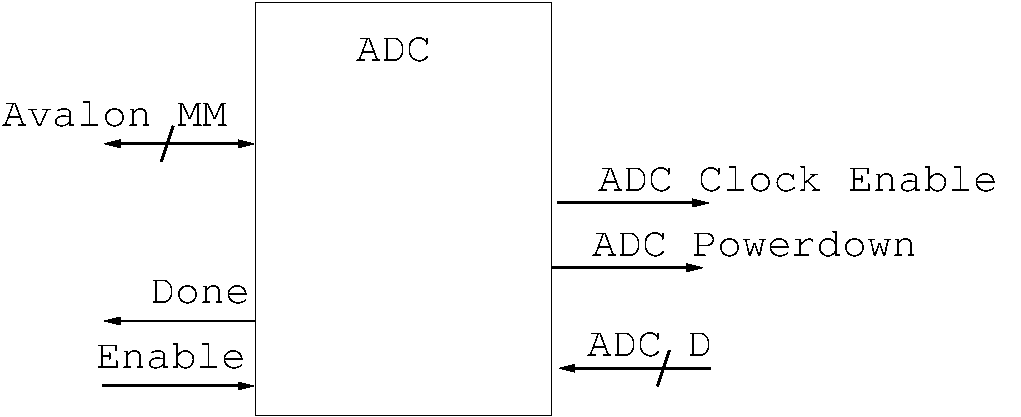
\includegraphics[width=0.4\textwidth]{adc_periph}
\caption{Black box overview of the ADC module}
\label{figure:adc_blackbox}
\end{center}
\end{figure}

The module is enabled by asserting the \texttt{enable} signal for one clock cycle. When
the module completes the sampling, it asserts the \texttt{done} signal until it is enabled
again.

The \texttt{enable} and \texttt{done} signals are connected to the ADC interface
in the SoPC, as described in the SoPC section.


Figure \ref{figure:state_adc} shows a simplified state diagram of the ADC module's state
machine. The module starts up in the \texttt{END} state. While in this state, the
ADC powerdown signal remains asserted, putting the ADC chip into low power mode. In this
state the ADC clock enable signal is deasserted, so that the clock to the ADC is gated.

\begin{figure}[h!]
\begin{center}
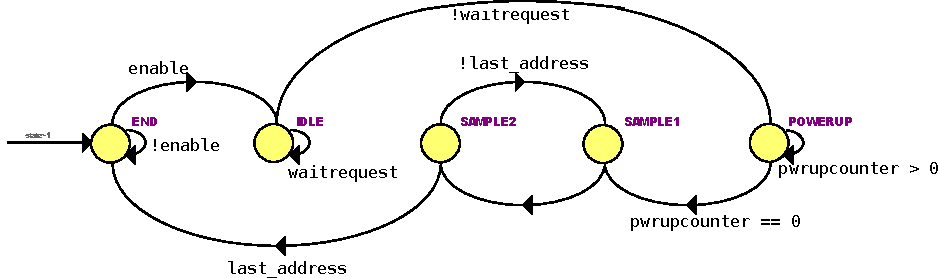
\includegraphics[width=\textwidth]{state_adc}
\caption{Simple state diagram of the ADC module}
\label{figure:state_adc}
\end{center}
\end{figure}

When the external \texttt{enable} signal is asserted, the module transitions into the
\texttt{IDLE} state, where it stays until the SRAM arbiter deasserts the \texttt{mem\_waitrequest}
signal. As soon as the SRAM is ready, the module transitions into the \texttt{POWERUP} state
which ensures that the ADC has enough time after deasserting the powerdown signal to
get back into normal operating mode.

After the ADC has fully powered up, the module transitions between the \texttt{SAMPLE1} and
\texttt{SAMPLE2} states, taking a sample during each and storing it into the upper and lower
bytes of a 16-bit register, respectively.

During the \texttt{SAMPLE2} state, this 16 bit register is written out to SRAM via the
Avalon MM interface to the SRAM arbiter.

As soon as the SRAM is full the module transitions back into the \texttt{END} state, in which
the \texttt{done} signal is asserted notifying the ADC interface in the SoPC that the ADC
module has finished sampling and the ADC is powered down.



